\documentclass[12pt]{article}
\usepackage{graphicx} % Required for inserting images
\usepackage{amsmath,amssymb,amsthm,amsfonts}
\usepackage{xcolor}
\usepackage{tasks}
%\usepackage{enumitem}
\usepackage[margin=2cm]{geometry}
\usepackage{tkz-euclide}

\usepackage[utf8]{inputenc}
\usepackage[T1]{fontenc}
\usepackage{amsmath}
\usepackage{amsfonts}
\usepackage{amssymb}
\usepackage[version=4]{mhchem}
\usepackage{stmaryrd}
\usepackage{enumerate}
\usepackage{multicol}
\usepackage{xcolor}
\usepackage{graphicx}
\usepackage{ulem}
\usepackage{cancel}
\usepackage{tikz}
\usepackage{tkz-euclide}
\usepackage[finnish]{babel}

%\usepackage[style=alphabetic,]{biblatex}

%\usepackage[margin=2cm]{geometry}

\newcommand{\brac}[1]{\left(#1\right)}
\newcommand{\sqbrac}[1]{\left[#1\right]}
\newcommand{\set}[1]{\left\{#1\right\}}

\newcommand{\dd}[0]{\mathrm{d}}
\newcommand{\dx}[0]{\mathrm{d}x}

\newcommand{\hatu}{\hat{u}}
\newcommand{\hatv}{\hat{v}}
\newcommand{\hatw}{\hat{w}}
\newcommand{\hatn}{\hat{n}}

\newcommand{\vu}{\overline{u}}
\newcommand{\vv}{\overline{v}}
\newcommand{\vw}{\overline{w}}
\newcommand{\vp}{\overline{p}}
\newcommand{\vn}{\overline{n}}

\newcommand{\va}{\overline{a}}
\newcommand{\vb}{\overline{b}}
\newcommand{\vc}{\overline{c}}
\newcommand{\vd}{\overline{d}}


\newcommand{\vi}{\hat{\imath}}
\newcommand{\vj}{\hat{\jmath}}
\newcommand{\vk}{\hat{k}}

\newcommand{\ratkaisu}[1]{\hfill{\color{blue}\quad\textrm{Ratkaisu: } #1}}

\newcommand{\ratkaisuu}[1]{{\color{blue}\textrm{Ratkaisu: } #1}}

\newcommand{\kaava}[1]{{\color{green!50!black}#1}}

%\renewcommand{\ratkaisu}[1]{}
%\renewcommand{\ratkaisuu}[1]{}
%\renewcommand{\kaava}[1]{}

\newcommand{\vihje}[1]{{\color{red}Vihje. #1}}
\newcommand{\extra}[0]{\textbf{Extra.}~}

\title{OAMK}
\author{Juha-Matti Huusko}
\date{August 2023}

\renewcommand{\ratkaisu}[1]{{\color{blue}\quad\textrm{Ratkaisu: } #1}}

\renewcommand{\ratkaisu}[1]{}

\begin{document}
\thispagestyle{empty}

\section*{Early exam, sample 2.9.2024}
\subsubsection*{Mathematics for Programmers, ID00EK08-3001}

\section*{Basic math}

\begin{enumerate}
\item 
(a) Simplify the expression
$$
\left(\frac{1}{7}-\frac{1}{10}\right)\bigg/\left(\frac{1}{7}+\frac{1}{2}\right)\ratkaisu{1/25}
$$
to the form $\frac{p}{q}$, where $p$ and $q$ are integers.

(b) Simplify by opening the parentheses
$$
(3x+2)^2-2(6x-2)+5.\ratkaisu{9x^2+13}
$$

\item (a) Solve the quadratic equation
$2x^2-8x+6=0$.%\ratkaisu{x=1 \textrm{ tai } x=3}$

(b) Solve the unknowns $x$ and $y$ from the pair of equations
$$
\begin{cases}
6x+7y&=4\\
x+2y&=2.
\end{cases}\ratkaisu{y=8/5, x=-6/5}
$$


\item (a) Solve $x$ when $5^{4x}=3^{x+2}$.

(b) Solve $x$ when $2\ln(3x)-\ln(x)=\ln(x+2)$.
\end{enumerate}

\newpage
\section*{Calculus}

\begin{enumerate}
\item Find $f'(x)$, when
\begin{enumerate}
\item $f(x)=4x^5-\sqrt{2x}+\frac{1}{x^3}$
\item $f(x)=2\sin(3x)-7e^{x^4}$
\item $f(x)=e^x\ln(x)$
\end{enumerate}
\begin{figure}[h!]
    \centering
\def\px{1}
\def\py{2}
\def\qx{4}
\def\qy{3}
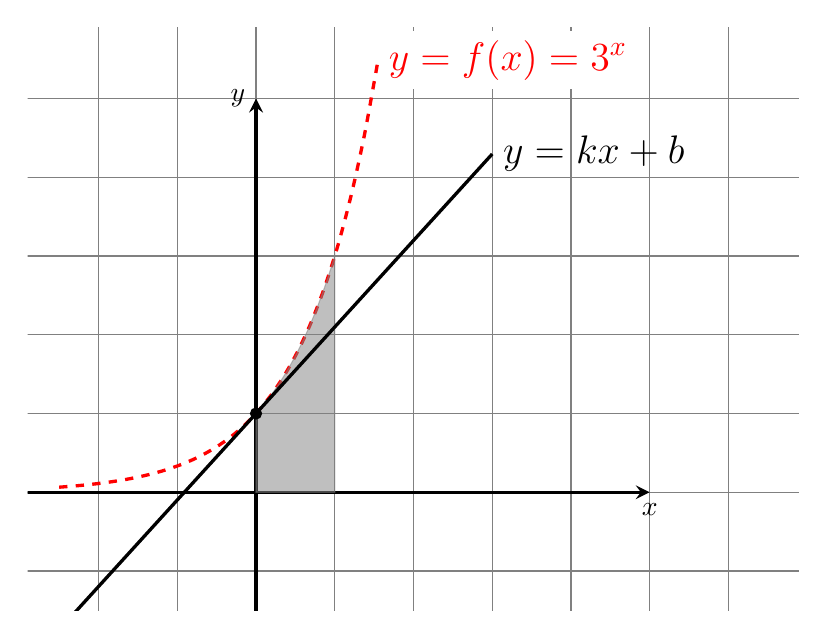
\begin{tikzpicture}[>=stealth]
\path[clip] (-2.9,-1.5) rectangle (6.9,5.9);
\draw[gray] (-6.9,-6.9) grid (6.9, 6.9);
\draw[very thick,->] (-5,0)--(5,0) node[below]{$x$};
\draw[very thick,->] (0,-5)--(0,5) node[left]{$y$};
%\draw[very thick, blue, domain=-2.5:2.5,smooth,variable=\t] plot ({\t},{1+0.693*\t+0.24*\t*\t});
\draw[very thick, red, dashed, domain=-2.5:1.55,smooth,variable=\t]
  plot ({\t},{exp(1.0986*\t)}) node[fill=white,right]{{\Large $y=f(x)=3^x$}};
\filldraw[gray, opacity=0.5, domain=0:1,smooth,variable=\t]
  plot ({\t},{exp(1.0986*\t)}) -- (1,0) --(0,0)--cycle;
\draw[very thick] (-3,-2.2958)--(3,4.2958) node[right]{{\Large $y=kx+b$}};
\filldraw (0,1) circle (2pt);
\end{tikzpicture}
    \caption{A graph of a function, a tangent line and a shaded area. Gridlines are one unit apart.}
    \label{fig:eksponentti-deri-int}
\end{figure}
\item Find the equation $y=kx+b$ of the line in Figure~\ref{fig:eksponentti-deri-int}.
\item Calculate the shaded area in Figure~\ref{fig:eksponentti-deri-int}.
\item  Find x > 0 which is the maximum of \(f(x)=x^8e^{-3x}\).
\item Calculate
\begin{enumerate}
\item $\int 4x+\sqrt{x}dx$
\item $\int \cos(2x)dx$
\item $\int_2^3 e^{-x}+1dx$
\end{enumerate}
\end{enumerate}

\newpage
\section*{Calculus formulas}

$$y-y_1=k(x-x_1),\quad y=kx+b,\quad k=\frac{y_2-y_1}{x_2-x_1}=f'(x_1)$$

$$
\int_a^b f(x)dx=\bigg |_a^b F(x)=F(b)-F(a),\quad F'(x)=f(x)
$$

$$
\begin{array}{rl|rl}
\textbf{Differentiation} && \textbf{Integration}&\\[2mm]
Dx^n&=nx^{n-1}     \qquad\qquad&\qquad\qquad\int x^ndx&=\frac{x^{n+1}}{n+1}+C \\[2mm]
De^x&=e^x &\int e^xdx&=e^x+C\\[2mm]
Db^x&=b^x\ln(b) & \int b^xdx&=\frac{b^x}{\ln(b)}\\[2mm]
D\ln(x)&=\frac{1}{x} &&\\[2mm]
D\ln|x|&=\frac{1}{x} &\int\frac{1}{x}dx&=\ln|x|+C\\[2mm]
D\log_a(x)&=\frac{1}{x\ln(a)} &&\\[2mm]
D\log_a|x|&=\frac{1}{x\ln(a)} &&\\[2mm]
D\sin(x)&=\cos(x)   &\int\cos(x)dx&=\sin(x)+C\\[2mm]
D\cos(x)&=-\sin(x)  &\int\sin(x)dx&=-\cos(x)+C\\[2mm]
D\tan(x)&=1+\tan^2(x) \qquad&\qquad\int 1+\tan^2(x)dx&=\tan(x)+C\\[2mm]

Dx\ln(x)-x&=\ln(x) & \int\ln(x)dx&=x\ln(x)-x+C\\[10mm]

D\arcsin(x)&=\frac{1}{\sqrt{1-x^2}} & \int\frac{1}{\sqrt{1-x^2}}&=\arcsin(x)+C\\
D\arccos(x)&=\frac{1}{-\sqrt{1-x^2}} & \int\frac{1}{-\sqrt{1-x^2}}&=\arccos(x)+C\\
D\arctan(x)&=\frac{1}{1+x^2} & \int\frac{1}{1+x^2}&=\arctan(x)+C\\

D\sinh(x)&=\cosh(x) &&\\
D\cosh(x)&=\sinh(x) &&\\
D\tanh(x)&=\frac{1}{\cosh^2(x)} &&\\
\end{array}  
$$
\vspace{1cm}
$$
\begin{array}{rl|rl}
\textbf{Differentiation} && \textbf{Integration}&\\[2mm]
D f(g(x))&=f'(g(x))g'(x) & \int f(g(x))g'(x)dx&=f(g(x))+C\\[2mm]
\textrm{Special cases} &&&\\
D\ln(f(x))&=\frac{f'(x)}{f(x)} & \int \frac{f'(x)}{f(x)}dx&=\ln(f(x))+C\\[2mm]
D e^{f(x)}&=e^{f(x)}f'(x) & \int f'(x)e^{f(x)}dx&=e^{f(x)}+C\\[10mm]
D fg&=f'g+fg'& \int f'g dx&=fg-\int fg'dx\\[2mm]
D (f/g)&=(gf'-fg')/g^2 &&\\[2mm]
\end{array}  
$$

\newpage
\section*{Basic formulas}

Fractions
$$
\frac{a}{b}+\frac{c}{d}=\frac{ad}{bd}+\frac{bc}{bd}
=\frac{ad+bc}{bd},\quad 
\frac{a}{b}\cdot\frac{c}{d}=\frac{ac}{bd},\quad
\frac{a}{b}\bigg/\frac{c}{d}=\frac{a}{b}\cdot\frac{d}{c}=\frac{ad}{bc}
$$
Powers
$$
a^ba^c=a^{b+c},\quad 
\frac{a^b}{a^c}=a^{b-c},\quad 
(a^b)^c=a^{bc},\quad 
(ab)^c=a^ba^c,\quad 
\brac{\frac{a}{b}}^c=\frac{a^b}{b^c}
$$
Roots
$$
(a^b)^{\frac{1}{b}}=a^{b\cdot \frac{1}{b}}=a^1=a,\quad\textrm{jos}\quad a>0,\quad 
\sqrt{a}=a^{\frac{1}{2}},\quad \sqrt[3]{a}=a^{\frac{1}{3}}
$$
First degree equation
$$
ax=b\quad\Leftrightarrow\quad x=\frac{b}{a}
$$
Quadratic equation
$$
ax^2+bx+c=0\quad\Leftrightarrow\quad x=\frac{-b\pm\sqrt{b^2-4ac}}{2a}
$$
System of linear equations
$$
\begin{cases}
ax+by&=U\\
cx+dy&=V
\end{cases}\quad\Rightarrow
\begin{cases}
acx+bcy&=cU\\
-acx+-ady&=-aV
\end{cases}\Rightarrow\ldots
$$

$$
\begin{cases}
ax+by&=U\\
cx+dy&=V
\end{cases}\quad\Rightarrow
y=\frac{U-ax}{b}\quad\Rightarrow
cx+d\frac{U-ax}{b}=V\Rightarrow\ldots
$$

$$
\begin{cases}
ax+by&=U\\
cx+dy&=V
\end{cases}\quad\Rightarrow
\begin{cases}
x&=\frac{Ud-bV}{ad-bc}\\
y&=\frac{aV-Uc}{ad-bc}
\end{cases}
$$
Function $f(x)$ and inverse function $g(x)=f^{-1}(x)$
$$
f(g(x))=x,\quad
g(f(x))=x
$$

$$\arraycolsep=1.4pt\def\arraystretch{1.5}
\begin{array}{rl|rl}
\textbf{Powers} && \textbf{Logarithms}\\
a^1 &=a & \log_a(a)&=1\\
a^0 &=1 & \log_a(1)&=0\\
a^b=c\quad\Leftrightarrow\quad a&=c^{\frac{1}{b}} & \log_a(c) &=\frac{1}{\log_c(a)}\\
a^ba^c &= a^{b+c} & \log_a(bc)&=\log_a(b)+\log_a(c)\\
\frac{a^b}{a^c}&=a^{b-c} & \log_a\frac{b}{c}&=\log_a(b)-\log_a(c)\\
(a^b)^c&=a^{bc} & \log_a(b)&=\frac{\log_c(b)}{\log_c(a)}\\
&& \log_a(b^c)&=c\log_a(b)\\
\end{array}
$$

\begin{equation*}
\begin{split}
\log_{10}(x)&\approx\frac{x-1}{x+1},\quad\frac{1}{5}\leq x\leq 5,\\
\log_{e}(x)&\approx 2\frac{x-1}{x+1},\quad\frac{1}{3}\leq x\leq 3,\\
\log_{2}(x)&\approx 3\frac{x-1}{x+1},\quad\frac{1}{2}\leq x\leq 2,\\
\end{split}
\end{equation*}

\(
\begin{array}{rlrlrl}
\log_2(2)&=1 &\qquad \log_2(e)&\approx 1.4427 &\qquad \log_2(10)&\approx 3.3219\\
\log_e(2)&\approx 0.6931 & \log_e(e)&=1 & \log_e(10)&\approx 2.3026\\
\log_{10}(2)&\approx 0.30103 & \log_{10}(e)&\approx 0.4343 & \log_{10}(10)&=1\\
\end{array}
\)
\vspace{5mm}

Powers
$$
a^ba^c=a^{b+c},\quad 
\frac{a^b}{a^c}=a^{b-c},\quad 
(a^b)^c=a^{bc},\quad 
(ab)^c=a^ba^c,\quad 
\brac{\frac{a}{b}}^c=\frac{a^b}{b^c}
$$

Logarithms
$$
\ln(ab)=\ln(a)+\ln(b),\quad
\ln(\frac{a}{b})=\ln(a)-\ln(b),\quad
\ln(a^b)=b\ln(a)
$$


\begin{equation*}
\begin{split}
\log_a(x)=y\quad&\Leftrightarrow\quad a^y=x
\end{split}
\end{equation*}


$$
\log_a(1)=0,\quad
\log_a(a)=1,\quad
\log_a(a^x)=x,\quad
a^{\log_a(x)}=x
$$

\begin{equation*}
\begin{split}
\log_a(b^c)&=c\log_a(b)\\
\log_a(xy)&=\log_a(x)+\log_a(y)\\
\log_a\left(\frac{x}{y}\right)
&=\log_a(x)-\log_a(y)\\
\log_a(x)&=\frac{\log_b(x)}{\log_b(a)}
\end{split}
\end{equation*}

$$
\textrm{lb}(x)=\log_2(x),\quad
\lg(x)=\log_{10}(x),\quad
\ln(x)=\log_e(x),\quad
e\approx 2,72
$$

Trigonometry

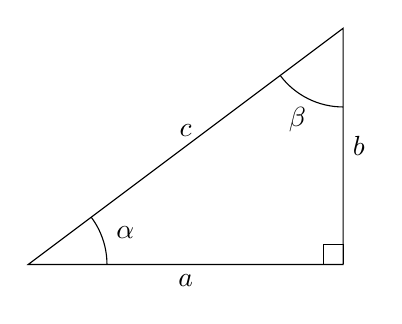
\begin{tikzpicture}
\draw (0,0) coordinate (o);
\draw (4,0) coordinate (u);
\draw (4,3) coordinate (v);
\draw (o)--(u) node[midway, below]{$a$}
--(v) node[midway, right]{$b$}
--(o) node[midway, above]{$c$} --cycle;
\tkzMarkRightAngle(o,u,v);
\tkzMarkAngle(o,v,u);
\tkzLabelAngle[pos=1.3](o,v,u){$\beta$};
\tkzMarkAngle(u,o,v);
\tkzLabelAngle[pos=1.3](u,o,v){$\alpha$};
\end{tikzpicture}

$$
c^2=a^2+b^2
$$

$$
\sin(\alpha)=\frac{b}{c},\quad
\cos(\alpha)=\frac{a}{c},\quad
\tan(\alpha)=\frac{b}{a},\quad
$$

$$
\alpha=\arcsin\frac{b}{c},\quad
=\arccos\frac{b}{c},\quad
=\arctan\frac{b}{c},\quad
$$

$$
\alpha=\textrm{imag}(\ln(a+bi))\cdot\frac{180^\circ}{\pi}
$$

\end{document}